\chapter{Expected Nodes: communautés de liens dans les graphes statiques}
\minitoc

Les structures communautaires dans les graphes ont été beaucoup étudiées lorsque la structure concerne les n\oe uds mais également, dans une moindre mesure, pour les liens.
Les partitions de n\oe uds d'un graphe trouvent leurs limites lorsque les communautés se chevauchent.
Dans ce cas, il est plus intéressant à ce que chaque n\oe uds puisse appartenir à plusieurs communautés.
On manipule alors une partition chevauchante ou couverture.
Pour répondre à ce problème de nombreux algorithmes ont été proposés pour la détection et l'évaluation de couvertures de n\oe uds.
Cependant les couvertures, en tant que généralisation des partitions, sont encore plus difficiles à évaluer que les partitions.
Les partitions de liens, quant à elles, restent des objets plus simple à manipuler.
De plus, elles permettent de mettre en avant une autre structure ayant également du sens.

Dans un réseau sociale, chaque personne a plusieurs centres d'intérêts: famille, sport, politique...
Lorsque deux personnes sont communiquent, la communication a lieu dans un contexte bien particulier.
Bien que les personnes ont plusieurs centres d'intérêts, la raison de la communication est unique.
Il semble donc qu'une information importante soit intrinsèquement liée au lien.
Via la recherche de partitions de liens d'un graphe, c'est cette information que nous cherchons à capturer.

Il apparait donc les partitions de liens sont des objets à part entières pertinent à étudier.
Il est alors nécessaire d'adapter les outils d'analyses pour évaluer directement les partitions de liens.
Nous développons ici une approche similaire à ce qui est fait pour les partitions de n\oe uds et la modularité~\cite{Newman2004}.
Le but est de créer une fonction de qualité permettant d'évaluer une partition de liens d'un graphe.


\section{Travaux existants}
Les notations utilisées sont les suivantes. Soit $G=(V,E)$ un graphe non-orienté avec $V$ l'ensemble des n\oe uds de taille $n$ et $E \subseteq V \times V$ l'ensemble des liens de taille $m$. 
Le degré d'un sommet $u$ de $G$ est noté $d_G(u)$.
Une partition des liens en $k$ groupes est notée $\mathcal{L}=(L_1,L_2,\ldots,L_k)$ avec $L_i \subseteq E \ \forall i$, $L_i\cap L_j=\emptyset \ \forall i\neq j$ et $\bigcup_i L_i=E$.
Pour un groupe de liens $L \in \mathcal{L}$, on pose $V_{in}=\{u \in V, \exists (u,v) \in L\}$ l'ensemble des n\oe uds internes au groupe $L$, $V_{out}=\{u \in V\setminus V_{in}, (u,v) \in E \wedge v \in V_{in} \}$ représente les n\oe uds adjacents au groupe $L$ et enfin $L_{out}=\{(u,v) \in E \setminus L, u \in V_{in} \vee v \in V_{in} \}$ l'ensemble des liens adjacents au groupe $L$ (voir Figure~\ref{fig:example_def_expected}).

\begin{figure}
\centering
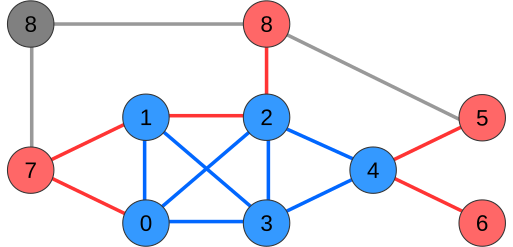
\includegraphics[width=0.4\linewidth]{img/ExpectedNodes/exemple2}
\caption{Exemple d'un groupe de liens $L$ (en \textcolor{semilightblue}{bleu}). Les liens \textcolor{pinkyred}{rouges} sont les liens adjacents $L_{out}$ connectant les n\oe uds internes $V_{in}$ (en \textcolor{semilightblue}{bleu}) aux n\oe uds adjacents $V_{out}$ (en  \textcolor{pinkyred}{rouge}).}
\label{fig:example_def_expected}
\end{figure}

Il existe différent type de méthodes existantes.
Il y les méthodes évaluant une partition de liens via la transformation de la partition en une couverture de n\oe uds~\cite{Huang2013,Lim2014,Wu2010a}.
Il serait tentant de considérer que les partitions de liens et les couvertures de liens sont équivalentes.
Ainsi pour évaluer une partition de liens, il suffirait de transformer la partition en couverture.
Or, ce changement n'est pas anodin.
D'une part, les couvertures de n\oe uds permettent de modéliser beaucoup plus de situations car il n'y a aucune contrainte sur les couvertures.
D'autre part, il n'est pas trivial de transformer une partition de liens en couverture de n\oe uds, et \emph{vice versa}.

\begin{figure}
\centering
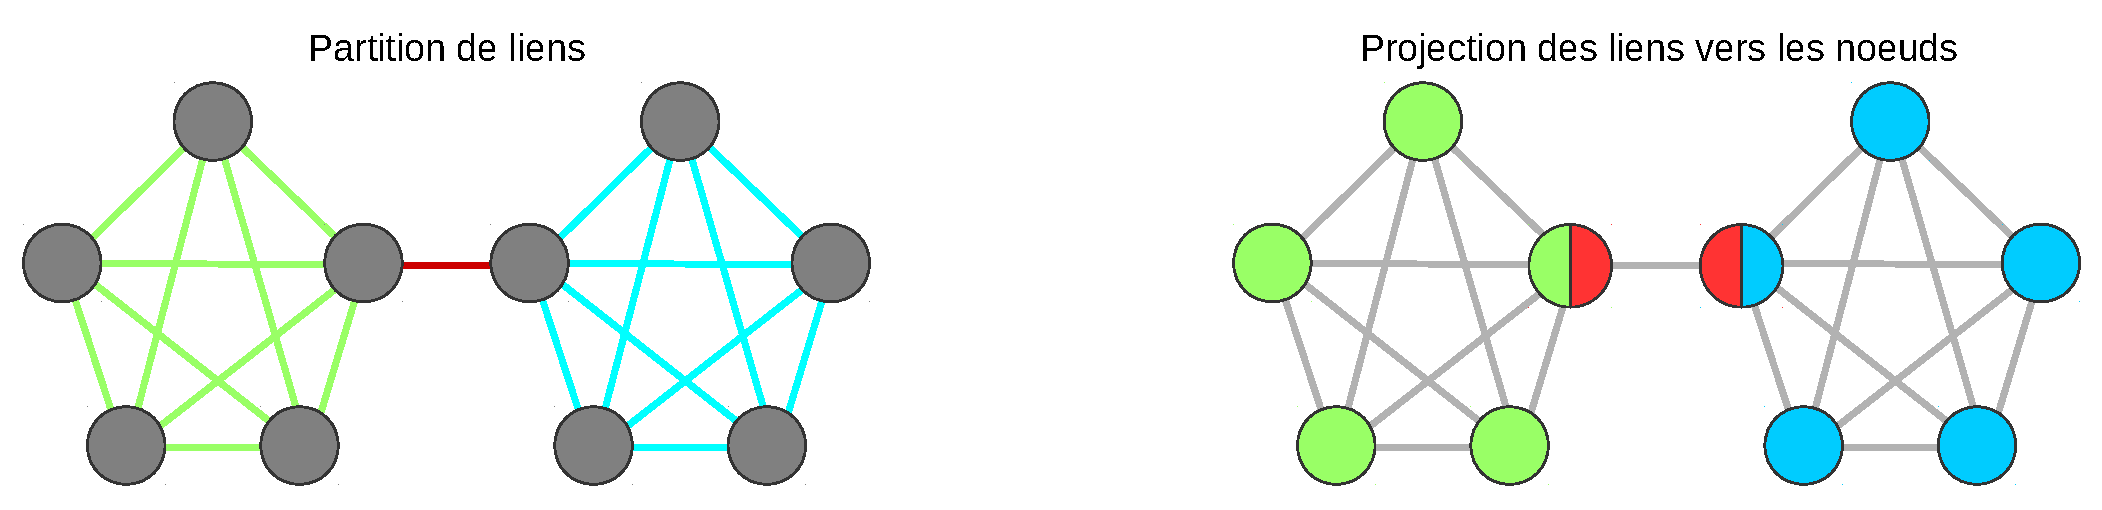
\includegraphics[width=0.9\linewidth]{img/ExpectedNodes/Partition_Couverture}
\caption{Transformation d'une partition de liens à gauche en couverture de n\oe uds à droite. La couleur représente un groupe.}
\label{fig:Partition_Couverture}
\end{figure}

Dans la figure~\ref{fig:Partition_Couverture}, est présenté une transformation basique d'une partition de liens en une couverture.
Dans cette transformation, un n\oe uds dans la couverture prends comme communauté l'ensemble des communautés de ses liens.
Dans cet exemple, il est évident que la communauté rouge consitutée des deux n\oe uds centraux n'est pas une communauté légitime et qu'il s'agit d'un artefact de la transformation.
La transformation d'une partition n'est donc pas un acte neutre.
Cet aspect a d'ailleurs était mis en avant par Esquivel~\emph{et al}~\ref{Esquivel2011}.
Face à ce problème, nos travaux ainsi que quelques méthodes existantes proposent des méthodes évaluant directement les partitions de liens.

Ahn \emph{et al.}~\cite{Ahn2010a} sont parmis les premiers à avoir proposé une méthode détectant les communautés de liens.
Leurs méthodes \emph{link clustering} est une méthode hiérarchique d'agglomération.
Elle construit un dendrogramme en agglomérant de manière itérative les groupes de liens en fonction de leurs similarités calculée par l'indice de Jaccard.
Afin de decider de la coupe du dendrogramme et de la partition résultantes, la fonction \emph{partition density} est utilisée.
Pour une partition de liens donnée $\mathcal{L}$, la \emph{partition density} est définie de la manière suivante:
\begin{equation}
D(\mathcal{L}) = \dfrac{\sum_{L \in \mathcal{L}} |L|D(L)}{m} \quad D(L) = \dfrac{|L|- min_D(|V_{in}|) }{max_D(|V_{in}|) - min_D(|V_{in}|)},
\end{equation}
Il s'agit de la moyenne pondéré de la qualité de chaque groupe.
La qualité d'un groupe est le nombre de liens du groupe normalisé par le nombre de liens minimum et maximum pour un groupe de $|V_{in}|$ n\oe uds.
Le nombre minimum de liens est obtenu par un arbre: $min_D(N) = N - 1$.
Le nombre maximum est obtenu par une clique: $max_D(N) = \dfrac{N(N - 1)}{2}$.\\
Aprés simplification, on obtiens la formule suivante:

\begin{equation}
 D(L) = 2 \dfrac{|L| - (|V_{in}|-1) }{(|V_{in}|-1) (|V_{in}|-2)}.
\end{equation}

D'autres chercheurs~\cite{Li2013,Shi2013} ont par la suite utilisé la \emph{partition density} comme fonction à optimiser dans un algorithme génétique.
Leurs solutions semblent pour l'instant difficile car leurs algorithme reposent sur de nombreux critères et limité à de petit graphes.

Par ailleurs, la \emph{partition density} ne peut pas être directement appliquée aux graphes pondérés.
Une première proposition a été faite par Kim~\cite{Kim2014}.


Evans~\emph{et al.}~\cite{Evans2009} propose trois fonctions de qualité pour évaluer les partitions de liens.
Leurs fonctions de qualité sont basées sur trois marches aléatoires qui se déroulent sur les liens du graphe.
L'approche est similaire à la modularité car la modularité peut également être définie à l'aide de marche aléatoire sur les n\oe uds du graphe~\cite{Delvenne2010}.
Leurs trois fonctions de qualités peuvent être calculées et optimisées sur le graphe mais les auteurs ont montré que l'on pouvait, de manière completement équivalente, utiliser la modularité sur des line graphe pondérés ($LG_1$, $LG_2$, $LG_3$).
Ainsi, il suffit de construire le line graphe approprié puis d'utiliser un algorithme existant d'optimisation de la modularité tel que l'algorithme de \emph{Louvain}~\cite{Blondel2008a}.
Un line graphe est un graphe où chaque lien du graphe initial est transformé en un n\oe uds dans le line graphe.
Deux n\oe uds du line graphe sont reliés si les liens correspondant ont au moins un n\oe uds en commun.

Pour construire les lines graphes  $LG_1$, $LG_2$ et $LG_3$, nous définissons $B\in \mathcal{M}_{n,m}$ la matrice d'incidence du graphe $G$: un élément $B_{i\alpha}$ de cette matrice $|V| \times |E|$ est égale à $1$ si le lien $\alpha$ est relié au n\oe uds $i$ et 0 sinon.
Les matrices $LG_1$, $LG_2$ et $LG_3$ sont alors définies de la manières suivantes:
\begin{center}
	\begin{tabular}{|c|c|c|c|}
		\hline  & $x=1$ & $x=2$ &  $x=3$\\ 
		\hline \rule{0pt}{1.8em} $LG_x(\alpha,\beta)$ & $B_{i\alpha}B_{i\beta} (1-\delta_{\alpha \beta})$ & $\sum_{i \in V, d_G(i)>1}\dfrac{B_{i\alpha}B_{i\beta}}{d(i)-1}$ & $\sum_{i,j \in V, d(i)d_G(j)>0}\dfrac{B_{i\alpha}A_{ij}B_{j\beta}}{d(i)d(j)}$ \\
		\hline 
	\end{tabular} 
\end{center}
Soit $k_x(\alpha)= \sum_{\beta}LG_x(\alpha,\beta)$ le degré pondéré dans le line graphe $LG_x$ du n\oe uds représantant le lien $\alpha$ et $W_x = \sum_{\alpha,\beta \in |E|}LG_x(\alpha,\beta)$ la somme des poids des liens. Pour $x \in \{1,2,3\}$, la fonction de qualité $Evans_x$ est définie de la manières suivante:
\begin{eqnarray}
Evans_x(\mathcal{L}) = \dfrac{1}{W_x} \sum_{L_i \in \mathcal{L}} \sum_{e_1,e_2 \in L_i^2} LG_x    (e_1,e_2) -  \dfrac{k_x(e_1) k_x(e_2)}{W}.
\end{eqnarray}

Kim \emph{et al.}~\cite{Kim2011} ont exploré une extension du concept \emph{Minimum Length Description} (MDL) introduit par Rosvall~\emph{et al.}~\cite{Rosvall2008} qui méthode provenant de la théorie de l'information.
Cette extension de la \emph{MDL} évalue directement une partition de liens, contrairement à l'extension proposée par Esquivel~\emph{et al.}~\cite{Esquivel2011}.
Un avantage de leur méthode est de pouvoir comparer l'avantage d'utiliser une partition de liens ou une partition de n\oe uds avec leur \emph{MDL} respective.
Cependant, leur méthode semble favoriser les communautés de liens que dans des cas très précis.


\section{Définition d'Expected Nodes}
\subsection{Calcul et optimisation}


\section{Comparaison}
\subsection{Cas du graphe complet}


\subsection{Graphe LFR}


\section{Conclusion}
